% =============================================================================
%  paper.tex -- From Natural Language to Verifiable Reasoning:
%                A Semantic-Reduction Framework for Reliable AI Mathematics
%
%  Compilation (single pass is sufficient; the bibliography is inlined):
%      pdflatex paper.tex        (or: xelatex paper.tex)
%  A BibTeX version of every entry is provided in references.bib for users
%  who prefer \bibliography-based toolchains. All citations in this document
%  resolve against the inline thebibliography below.
% =============================================================================
\documentclass[11pt]{article}

\usepackage[T1]{fontenc}
\usepackage[margin=1in]{geometry}
\usepackage{amsmath,amssymb,amsthm}
\usepackage{graphicx}
\usepackage{xcolor}
\usepackage{booktabs}
\usepackage{enumitem}
\usepackage{tikz}
\usetikzlibrary{arrows.meta,positioning}
\usepackage[hidelinks]{hyperref}

\newcommand{\den}[1]{[\![#1]\!]}
\newcommand{\Nat}{\mathbb{N}}
\newcommand{\accept}{\mathsf{accept}}
\newcommand{\reject}{\mathsf{reject}}

\theoremstyle{definition}
\newtheorem{definition}{Definition}[section]
\theoremstyle{plain}
\newtheorem{proposition}{Proposition}[section]
\theoremstyle{remark}
\newtheorem{remark}{Remark}[section]

\title{\bfseries From Natural Language to Verifiable Reasoning:\\[0.3em]
       A Semantic-Reduction Framework for Reliable AI Mathematics}
\author{AI4Math Reliability Working Group}
\date{\today}

\begin{document}
\maketitle

\begin{abstract}
Large language models (LLMs) now produce fluent and plausible mathematics, yet their
natural-language derivations cannot be checked directly: the same surface text may hide an
invalid inference, a hallucinated lemma, or a silent type coercion. We argue that reliability
cannot be recovered by post-hoc answer checking alone, because such checking has no formal
handle on the reasoning itself. We introduce a three-layer model of AI-mathematical
reliability---\emph{generation}, \emph{semantic reduction}, and \emph{verification}---and
identify semantic reduction, the translation of natural-language reasoning into a typed
intermediate representation (IR), as the critical bottleneck. We then present a
semantic-reduction framework comprising a typed IR, a
generation$\to$IR$\to$verification$\to$rendering pipeline, and bidirectional alignment
between IR and language for interpretability and traceability. We formalize a
\emph{verifiability gap} that quantifies the fraction of model outputs for which a verifier
provides no signal, and we contribute a taxonomy and a reliability checklist for
AI-for-mathematics systems. The framework is illustrated with a worked arithmetic example
and a formal-induction case. Our contribution is not a new prover but a lens: we elevate
semantic reduction from an incidental preprocessing step to a first-class, measurable system
component. We state our conclusions with explicit boundaries on scope.
\end{abstract}

\section{Introduction}
Large language models have made rapid progress on mathematical tasks. Trained models and
prompting techniques now solve a substantial fraction of grade-school word problems in
GSM8K~\cite{cobbe2021}, competition problems in MATH~\cite{hendrycks2021}, and
quantitative-reasoning benchmarks via systems such as Minerva~\cite{lewkowycz2022} and
GPT-4~\cite{achiam2023}. These systems are built on the Transformer architecture~\cite{vaswani2017} and
the few-shot scaling paradigm~\cite{brown2020}. Chain-of-thought prompting~\cite{wei2022} and
self-consistency~\cite{wang2023selfconsistency} further improved accuracy by exposing
intermediate steps.

These gains, however, come with a well-documented failure mode: models emit
\emph{plausible but incorrect} reasoning~\cite{bubeck2023,frieder2023,collins2024}. Because
the derivation is expressed in natural language, it has no type, no formal semantics, and no
checkable structure. A verifier cannot ask ``is this step valid?'' in a mechanical sense; it
can only ask ``is this final answer equal to the reference?''.

The AI-for-mathematics (AI4Math) community has responded with three broad strategies:
(i)~search and verification, in which sampled answers are scored by learned verifiers or
majority voting~\cite{cobbe2021,wang2023selfconsistency,lightman2024};
(ii)~formalization, in which proofs are checked by interactive theorem provers such as
Lean~\cite{demoura2015,demoura2021} and the correctness is absolute; and
(iii)~reproducible evaluation, in which benchmarks and protocols are standardized so claims can
be audited~\cite{hendrycks2021,zheng2022}. Each strategy attacks a real symptom, but none
makes explicit the shared structural problem underneath: \emph{between the natural-language
derivation and the formal verifier there is a translation step whose instability determines
whether verification is even possible.}

Our thesis is that reliability cannot be recovered solely by \emph{final} verification.
Instead, a dedicated \emph{semantic-reduction layer} must sit between generation and
verification, converting informal reasoning into a typed, machine-checkable object. When this
layer fails, verification has no anchor and hallucinations cannot be detected; when it
succeeds, verification becomes a routine, auditable operation. This paper makes the following
contributions:
\begin{itemize}[leftmargin=1.5em]
  \item A \textbf{three-layer model} of AI4Math reliability (generation / semantic reduction /
        verification) that makes the translation step explicit (\S\ref{sec:model}).
  \item A \textbf{semantic-reduction framework} with a typed IR, a four-stage pipeline, and
        bidirectional IR--language alignment (\S\ref{sec:framework}).
  \item A formal notion of the \textbf{verifiability gap}, quantifying the outputs on which a
        verifier is silent, together with a \textbf{taxonomy} and a \textbf{reliability
        checklist} for AI4Math systems (\S\ref{sec:analysis}).
\end{itemize}
We emphasize the boundary of this work: we do not train a new model, build a new prover, or
run a large benchmark. We provide a conceptual and formal lens, with worked micro-examples,
intended to make reliability properties of AI4Math systems \emph{measurable} and
\emph{auditable}.

\section{Related Work}\label{sec:related}
\paragraph{Generation and prompting.}
Chain-of-thought prompting elicits intermediate reasoning and improves accuracy on
multi-step problems~\cite{wei2022}. Self-consistency reduces variance by sampling many chains
and taking a majority vote~\cite{wang2023selfconsistency}. Benchmark-driven progress is
tracked on GSM8K~\cite{cobbe2021} and MATH~\cite{hendrycks2021}; domain-tuned models such as
Minerva~\cite{lewkowycz2022} and general models such as GPT-4~\cite{achiam2023} show strong but
imperfect performance, with systematic errors on interaction-heavy tasks~\cite{collins2024}.

\paragraph{Post-hoc verification.}
Learned outcome verifiers score candidate solutions to select an answer~\cite{cobbe2021}.
Process-supervision rewards individual steps rather than only the final answer, improving
step-level reliability~\cite{lightman2024}. Program-aided approaches sidestep free-form
reasoning by having the model emit executable code (``program-of-thought''), which is then run
by an interpreter~\cite{gao2023pal}. These methods verify an \emph{answer} or a
\emph{program}, but they do not verify the \emph{claim that the program means what the problem
asked}; that meaning is left implicit in natural language.

\paragraph{Formal proof.}
Interactive theorem provers such as Lean offer a small, trusted kernel: once a proof is
accepted, its correctness follows from the axioms~\cite{demoura2015,demoura2021}. The
formulae-as-types correspondence~\cite{howard1980} grounds the idea that a proof is itself a
computable object, which motivates treating proofs as typed IR. Autoformalization uses LLMs to
translate informal mathematics into formal statements~\cite{wu2022}, and miniF2F provides a
cross-system benchmark of formally stated olympiad problems~\cite{zheng2022}. The
AlphaProof system combines a large proof-search policy with Lean so that every output is a
machine-checked proof; it reached a silver-medal standard (28 out of 42 points, solving four of six problems) on
IMO 2024~\cite{hubert2025}. These systems are powerful but exhibit a division of labor:
the neural component explores, while the kernel verifies---and the informal-to-formal
translation remains the fragile joint between them.

\paragraph{Neuro-symbolic discovery.}
Beyond solving fixed problems, hybrid systems have produced new mathematics: guiding human
intuition about knot invariants~\cite{davies2021}, discovering faster matrix-multiplication
algorithms with AlphaTensor~\cite{fawzi2022}, synthesizing solutions to olympiad geometry
without human demonstrations in AlphaGeometry~\cite{trinh2024}, and evolving programs that
yield new constructions in FunSearch~\cite{romera2024}. In each case the final artifact is
symbolic and independently checkable; the LLM supplies candidates.

\paragraph{Positioning.}
Across all of these lines of work, a common step recurs: informal or sampled output must be
mapped to a checkable object. We argue this step---\emph{semantic reduction}---deserves to be
named, modeled, and measured as a first-class component, rather than treated as an incidental
preprocessing detail. That is the position the present paper occupies.

\section{A Three-Layer Reliability Model}\label{sec:model}
We model an AI4Math pipeline as the composition of three layers, each with a distinct
responsibility and failure mode.

\begin{definition}[Three-layer model]
A \emph{reliable AI-mathematical reasoning system} is a triple
$(\mathrm{Gen}, \rho, \mathrm{Ver})$ where
\begin{enumerate}[label=(\roman*)]
  \item $\mathrm{Gen}$ is the \emph{generation layer}: a probabilistic map from a problem
        statement to a natural-language derivation $d$;
  \item $\rho$ is the \emph{semantic-reduction layer}: a partial map
        $\rho : \mathrm{NL} \rightharpoonup \mathrm{IR}$ from derivations to typed
        intermediate representations;
  \item $\mathrm{Ver}$ is the \emph{verification layer}: a function
        $\mathrm{Ver} : \mathrm{IR} \to \{\accept, \reject\}$ that checks an IR object against
        a formal statement $\varphi$.
\end{enumerate}
\end{definition}

\paragraph{Generation layer.}
The generation layer produces natural-language chains of reasoning (e.g., chain-of-thought).
Its defining properties are that it is \emph{probabilistic}, \emph{untyped}, and
\emph{informal}: tokens are not subject to any typing discipline, and validity is not a
property of the output format.

\paragraph{Semantic-reduction layer.}
The reduction layer maps a derivation to one of several equivalent formal objects: a formula in
first- or higher-order logic, a program in a domain-specific language, a proof object, or a
typed intermediate representation. Its theoretical grounding is the formulae-as-types
correspondence~\cite{howard1980}, which identifies proofs with computable objects of a
specified type. The layer faces three intrinsic challenges:
\begin{itemize}[leftmargin=1.5em]
  \item \emph{Ambiguity:} one natural-language sentence admits several formal readings.
  \item \emph{Missing typing:} informal quantities often lack an explicit type, so coercions
        are silently inserted.
  \item \emph{Non-invertibility:} the map $\rho$ is not surjective and, in general, not
        injective; one cannot reconstruct the intended meaning from the IR alone.
\end{itemize}

\paragraph{Verification layer.}
Given a typed IR object and a formal statement $\varphi$, the verifier checks: consistency
(no contradiction with the axioms), derivability (the object is a well-formed proof of
$\varphi$), factual grounding (any external facts used are declared), and constraint
satisfaction (side conditions hold). In a trusted-kernel prover such as Lean, acceptance means
the proof reduces to the axioms~\cite{demoura2015,demoura2021}.

\subsection{The Bottleneck: Semantic Reduction}
We claim that the dominant source of failure in current systems is the \emph{second} layer, not
the first or the third. The argument is structural. The verifier can only operate on
\emph{computable} objects (typed terms, programs, proof terms). If the reduction $\rho$ is
undefined on a derivation---because the sentence is ambiguous, a type is missing, or the
mapping is not invertible---then there is \emph{no handle to verify}. In that case the
verifier contributes no information: it cannot certify correctness, and it cannot detect a
hallucination that happens to be phrased fluently.

This explains two commonly observed phenomena. First, learned answer-verifiers improve
selection but leave step-level errors intact, because they score the surface rather than a
reduced object~\cite{cobbe2021,lightman2024}. Second, formal systems achieve absolute
reliability on the (often small) subset of problems that survive formalization, because the
reduction has succeeded there~\cite{hubert2025}. The reliability of the \emph{whole} system is
therefore governed by the coverage and fidelity of $\rho$.

\section{The Semantic-Reduction Framework}\label{sec:framework}
\subsection{Typed Intermediate Representation}
We propose that the reduction layer target a single, uniform typed IR. The IR is characterized
by four components:
\begin{itemize}[leftmargin=1.5em]
  \item a \emph{type system} assigning each object a type $\tau$;
  \item an \emph{operational semantics} $\den{\cdot} : \mathrm{IR} \to \mathrm{Value}$ giving
        each closed object a deterministic meaning;
  \item a \emph{constraint system} recording side conditions (e.g., ``divisor nonzero'');
  \item a \emph{compositional structure} (an abstract syntax tree or a workflow graph) so that
        sub-derivations can be checked independently and composed.
\end{itemize}
Concrete realizations include domain-specific languages, abstract syntax trees, proof objects,
and workflow graphs; they are interchangeable as long as they expose the four components above.

\subsection{Pipeline Architecture}
The framework instantiates a standard pipeline:
\[
\resizebox{\linewidth}{!}{$\displaystyle
\text{Natural language (LLM)}
\;\xrightarrow{\;\rho\;}\;
\text{Typed IR}
\;\xrightarrow{\;\mathrm{Ver}\;}\;
\text{Formal verification}
\;\xrightarrow{\;\mathrm{render}\;}\;
\text{Natural-language rendering}.$}
\]
The key design decision is that natural language is used only as an \emph{interface}, while
the IR is the \emph{execution core}: all checking happens on the IR, and the natural-language
text is re-rendered from the checked object.

\begin{figure}[t]
\centering
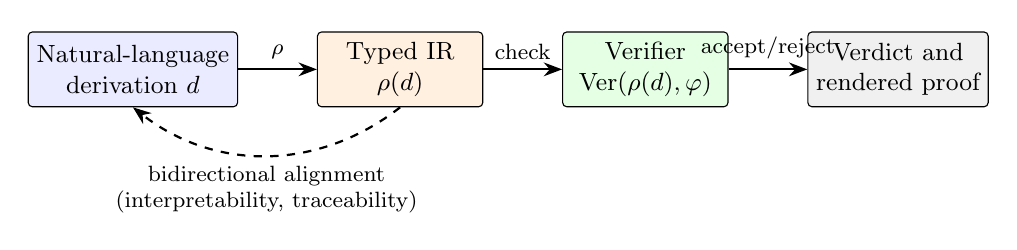
\begin{tikzpicture}[
  node distance=1.0cm and 1.0cm,
  box/.style={draw, rounded corners=1.5pt, align=center,
              minimum height=9.5mm, minimum width=2.1cm, inner sep=3pt, fill=#1, font=\small},
  arr/.style={-{Stealth}, thick}
]
\node[box=blue!8]   (nl)  {Natural-language\\derivation $d$};
\node[box=orange!12](ir)  [right=of nl] {Typed IR\\$\rho(d)$};
\node[box=green!10] (vf)  [right=of ir] {Verifier\\$\mathrm{Ver}(\rho(d),\varphi)$};
\node[box=gray!12]  (out) [right=of vf] {Verdict and\\rendered proof};
\draw[arr] (nl)  -- node[above,font=\footnotesize]{$\rho$} (ir);
\draw[arr] (ir)  -- node[above,font=\footnotesize]{check} (vf);
\draw[arr] (vf)  -- node[above,font=\footnotesize]{accept/reject} (out);
\draw[arr,dashed,bend left=38] (ir.south) to
      node[below,font=\footnotesize,align=center]{bidirectional alignment\\(interpretability, traceability)} (nl.south);
\end{tikzpicture}
\caption{The four-stage pipeline. Natural language is the interface; the typed IR is the
execution core on which all verification operates. The dashed arc denotes bidirectional
IR--language alignment.}
\label{fig:pipeline}
\end{figure}

\subsection{Bidirectional Alignment}
Reliability of the pipeline requires more than a forward reduction. We impose
\emph{bidirectional alignment} between IR and language, formalized as two requirements.
\begin{itemize}[leftmargin=1.5em]
  \item \emph{Interpretability:} the rendering map $\mathrm{render}$ is such that a human
        reading the rendered text can recover the intended structure of the IR; and
  \item \emph{Traceability:} each rendered claim carries a pointer back to the IR node that
        justified it, so any accepted or rejected step can be audited.
\end{itemize}
These requirements convert ``the model said so'' into ``the checked object at node $n$ says
so,'' which is the property that makes the output suitable for scholarly use.

\subsection{A Worked Example}\label{sec:example}
Consider the word problem ``Alice has $5$ apples and Bob gives her $3$ more; how many apples
does Alice have now?'' Let $\Gamma = \{a : \mathsf{Nat},\, b : \mathsf{Nat}\}$. The reduction
produces the typed program
\[
\rho(d) \;=\; \mathsf{let}\ a=5\ \mathsf{in}\ \mathsf{let}\ b=3\ \mathsf{in}\ a + b,
\]
typed by the rule
\[
\frac{\Gamma \vdash a : \mathsf{Nat} \qquad \Gamma \vdash b : \mathsf{Nat}}
      {\Gamma \vdash a + b : \mathsf{Nat}}\,(\mathsf{+}),
\]
with operational meaning $\den{a+b} = \den{5+3} = 8$, and the verifier checks
$\den{\rho(d)} = 8$ against the intended statement $\varphi$. The same problem also shows the
bottleneck. The sentence ``Alice gives away \emph{half} of her apples'' reduces only if
``half'' is mapped to a typed operation; if it is silently coerced to integer division
$5 / 2$, the verifier certifies the value $2$ while the intended meaning---that a half of five
whole apples is not a whole number---has been lost. The error is invisible to the verifier
precisely because it occurred during reduction, before any checkable object existed.

As a formal case, let $P(n) := (n + 0 = n)$ over $\Nat$. A derivation that first establishes
$P(0)$ and then $P(k) \Rightarrow P(k+1)$ for arbitrary $k$ reduces to the induction object
\[
\frac{P(0) \qquad \forall k.\; P(k) \Rightarrow P(k+1)}
      {\forall n.\; P(n)}\,(\text{induction on }\Nat),
\]
which in a dependently typed kernel corresponds to the recursor $\mathsf{Nat.rec}$. The typed
IR carries the proof as an object, and the verifier need only check the two premises.

\section{Analysis: A Verifiability Gap, a Taxonomy, and a Checklist}\label{sec:analysis}
\subsection{The Verifiability Gap}
Let $D$ be the set of derivations generated for a benchmark, and $D^{*} \subseteq D$ the
correct ones. A derivation $d$ is \emph{verifiable} if $\rho(d)$ is defined; write
$V = \{\,d \in D : \rho(d)\ \text{defined}\,\}$. The \emph{verifiability gap} is
\[
g \;=\; 1 - \frac{|V|}{|D|},
\]
the fraction of outputs on which the verifier is silent. We then have the following simple
but useful fact.

\begin{proposition}
Let $\mathrm{Ver}$ be sound for a statement $\varphi$: if
$\mathrm{Ver}(\rho(d),\varphi) = \accept$ then $d$ is a correct proof of $\varphi$. Then
(i)~among accepted outputs, correctness is guaranteed (no false positives); and
(ii)~all errors lying in $D \setminus V$ are \emph{undetectable} by $\mathrm{Ver}$, regardless
of how fluent they appear.
\end{proposition}

\begin{proof}[Proof sketch]
(i) is exactly soundness. For (ii), if $d \notin V$ then $\rho(d)$ is undefined, so
$\mathrm{Ver}$ receives no object and returns no signal; no computation of $\mathrm{Ver}$ can
distinguish a correct $d$ from an incorrect one in this set. \qedhere
\end{proof}

The proposition makes precise a design implication: the only lever that reduces silent error
is to shrink $g$ by enlarging $V$---that is, by improving $\rho$---not by improving
$\mathrm{Ver}$.

\subsection{A Taxonomy of Reliability Mechanisms}
Table~\ref{tab:taxonomy} classifies the dominant AI4Math approaches by \emph{where}
verification occurs and \emph{what} is verified. The taxonomy exposes a spectrum: answer
checking verifies a scalar at the end; program execution verifies a meaning only if the
program's intended denotation has been established; proof checking verifies the entire object
but depends entirely on a successful reduction.

\begin{table}[t]
\centering
\small
\begin{tabular}{@{}l l l l@{}}
\toprule
\textbf{Approach} & \textbf{Where verification occurs} & \textbf{What is verified} & \textbf{Dominant failure}\\
\midrule
Chain-of-thought \cite{wei2022} & none (surface only) & nothing formal & undetected wrong step\\
Outcome verifier \cite{cobbe2021} & after generation & final answer & step errors survive\\
Self-consistency \cite{wang2023selfconsistency} & after sampling & answer by majority & correlated errors\\
Program-of-thought \cite{gao2023pal} & at execution & program output & wrong program meaning\\
Autoformalization \cite{wu2022} & at reduction & formal statement & reduction infidelity\\
Proof kernel \cite{demoura2021,hubert2025} & throughout & proof object & coverage of $\rho$\\
\bottomrule
\end{tabular}
\caption{A taxonomy of reliability mechanisms along two axes: where verification occurs and
what is verified.}
\label{tab:taxonomy}
\end{table}

\subsection{A Reliability Checklist}
We distill the framework into a practical checklist for reporting and reviewing AI4Math
systems, inspired by but distinct from ML reproducibility checklists. Each item is an
\emph{auditable} property of the pipeline rather than a claim about accuracy.
\begin{enumerate}[leftmargin=1.5em]
  \item \textbf{Statement grounding.} Is the intended statement $\varphi$ formalized, or only
        paraphrased?
  \item \textbf{Reduction coverage.} What fraction of outputs admit a typed reduction (i.e.,
        what is $1-g$)?
  \item \textbf{Verifier soundness.} Is the checking kernel small, trusted, and audited?
  \item \textbf{Traceability.} Can each rendered step be traced to an IR node?
  \item \textbf{Reproducibility.} Are data, prompts, seeds, and evaluation protocol published?
  \item \textbf{Failure reporting.} Are unverifiable outputs reported rather than silently
        dropped?
  \item \textbf{Applicability boundary.} Does the system declare the problem classes it covers?
\end{enumerate}

\section{Limitations}\label{sec:limitations}
\paragraph{Design and coverage.}
The framework inherits the cost of its central component. Designing a typed IR with the four
required properties is nontrivial, and mapping natural language into it remains expensive and
imperfect; these are exactly the ambiguity, missing-typing, and non-invertibility challenges
of \S\ref{sec:model}. The framework is also \emph{conceptual}: it does not by itself produce
proofs, and our worked examples are micro-instances chosen for clarity rather than a
large-scale evaluation.

\paragraph{Threats to validity.}
The verifiability gap $g$ is only meaningful relative to a fixed reduction $\rho$ and
benchmark $D$; different choices of IR change $g$ even when the underlying model is unchanged.
We therefore treat $g$ as a \emph{comparative} diagnostic within one pipeline, not an absolute
quality measure. The proposition's conclusion is conditional on soundness, which must be
established separately for each verifier.

\section{Discussion and Future Work}\label{sec:discussion}
Three directions follow naturally. First, the IR can serve as the action space of a
proof-search agent, making the reduction and the search a single learned loop---as
AlphaProof-style systems implicitly do~\cite{hubert2025}. Second, the taxonomy and checklist
can be turned into a standardized reporting form for AI4Math papers, improving reproducible
evaluation~\cite{hendrycks2021,zheng2022}. Third, bidirectional alignment suggests training
objectives that reward round-tripping (language$\to$IR$\to$language), so that reduction
fidelity is optimized directly rather than as a byproduct of end-task accuracy.

\section{Conclusion}
We have argued that the reliability of AI mathematical reasoning is governed by a layer that
is rarely named and rarely measured: the \emph{semantic reduction} from natural language to a
typed, checkable object. We contributed a three-layer model that makes this layer explicit, a
semantic-reduction framework with a typed IR and a four-stage pipeline with bidirectional
alignment, and a formal notion of the verifiability gap together with a taxonomy and a
reliability checklist. The core claim is succinct: reliable AI reasoning requires
\emph{generation} plus \emph{semantic reduction} plus \emph{verification}, and any system
that omits or ignores the middle layer will silently fail on precisely the outputs it cannot
formalize. We have stated the boundary of this claim explicitly: it is a structural,
diagnostic lens, validated by construction and by worked examples, rather than a trained
system or a benchmark result. Future work will instantiate the framework on a fixed
benchmark to measure reduction coverage in practice.

% -------------------------- References (inlined) -----------------------------
\begin{thebibliography}{99}\small

\bibitem{howard1980}
W.~A. Howard.
The formulae-as-types notion of construction.
In \emph{To H.~B. Curry: Essays on Combinatory Logic, Lambda Calculus and Formalism},
J.~P. Seldin and J.~R. Hindley (eds.), Academic Press, pp.~479--490, 1980.

\bibitem{vaswani2017}
A. Vaswani, N. Shazeer, N. Parmar, J. Uszkoreit, L. Jones, A.~N. Gomez, L. Kaiser, and
I. Polosukhin.
Attention is all you need.
In \emph{Advances in Neural Information Processing Systems 30 (NeurIPS)}, 2017.

\bibitem{brown2020}
T.~B. Brown et al.
Language models are few-shot learners.
In \emph{Advances in Neural Information Processing Systems 33 (NeurIPS)}, 2020.

\bibitem{wei2022}
J. Wei, X. Wang, D. Schuurmans, M. Bosma, B. Ichter, F. Xia, E.~H. Chi, Q.~V. Le, and
D. Zhou.
Chain-of-thought prompting elicits reasoning in large language models.
In \emph{Advances in Neural Information Processing Systems 35 (NeurIPS)}, 2022.

\bibitem{cobbe2021}
K. Cobbe, V. Kosaraju, M. Bavarian, M. Chen, H. Jun, L. Kaiser, M. Plappert, J. Tworek,
J. Hilton, R. Nakano, C. Hesse, and J. Schulman.
Training verifiers to solve math word problems.
arXiv:2110.14168, 2021.

\bibitem{hendrycks2021}
D. Hendrycks, C. Burns, S. Kadavath, A. Arora, S. Basart, E. Tang, D. Song, and J. Steinhardt.
Measuring mathematical problem solving with the MATH dataset.
In \emph{Advances in Neural Information Processing Systems 34 Datasets and Benchmarks Track},
2021. arXiv:2103.03874.

\bibitem{lewkowycz2022}
A. Lewkowycz et al.
Solving quantitative reasoning problems with language models.
In \emph{Advances in Neural Information Processing Systems 35 (NeurIPS)}, 2022.
arXiv:2206.14858.

\bibitem{wang2023selfconsistency}
X. Wang, J. Wei, D. Schuurmans, Q. Le, E. Chi, S. Narang, A. Chowdhery, and D. Zhou.
Self-consistency improves chain of thought reasoning in language models.
In \emph{International Conference on Learning Representations (ICLR)}, 2023.
arXiv:2203.11171.

\bibitem{lightman2024}
H. Lightman, V. Kosaraju, Y. Burda, H. Edwards, B. Baker, T. Lee, J. Leike, J. Schulman,
I. Sutskever, and K. Cobbe.
Let's verify step by step.
In \emph{International Conference on Learning Representations (ICLR)}, 2024.
arXiv:2305.20050.

\bibitem{gao2023pal}
L. Gao, A. Madaan, S. Zhou, U. Alon, P. Liu, Y. Yang, J. Callan, and G. Neubig.
PAL: Program-aided language models.
In \emph{International Conference on Machine Learning (ICML)}, 2023. arXiv:2211.10435.

\bibitem{achiam2023}
J. Achiam et al.
GPT-4 technical report.
arXiv:2303.08774, 2023.

\bibitem{bubeck2023}
S. Bubeck et al.
Sparks of artificial general intelligence: Early experiments with GPT-4.
arXiv:2303.12712, 2023.

\bibitem{frieder2023}
S. Frieder, L. Pinchetti, R.-R. Griffiths, T. Salvatori, T. Lukasiewicz, P. Petersen,
and J. Berner.
Mathematical capabilities of ChatGPT.
In \emph{Advances in Neural Information Processing Systems 36 (NeurIPS)}, 2023.

\bibitem{davies2021}
A. Davies, P. Veli\v{c}kovi\'c, L. Buesing, S. Blackwell, D. Zheng, N. Toma\v{s}ev,
R. Tanburn, P. Battaglia, C. Blundell, A. Juh\'asz, et al.
Advancing mathematics by guiding human intuition with AI.
\emph{Nature}, 600(7887):70--74, 2021.

\bibitem{fawzi2022}
A. Fawzi, M. Balog, A. Huang, T. Hubert, B. Romera-Paredes, M. Barekatain, A. Novikov,
F.~J.~R. Ruiz, J. Schrittwieser, G. Swirszcz, et al.
Discovering faster matrix multiplication algorithms with reinforcement learning.
\emph{Nature}, 610(7930):47--53, 2022.

\bibitem{trinh2024}
T.~H. Trinh, Y. Wu, Q.~V. Le, H. He, and T. Luong.
Solving olympiad geometry without human demonstrations.
\emph{Nature}, 625(7995):476--482, 2024.

\bibitem{romera2024}
B. Romera-Paredes, M. Barekatain, A. Novikov, M. Balog, M.~P. Kumar, E. Dupont,
F.~J.~R. Ruiz, J.~S. Ellenberg, P. Wang, O. Fawzi, et al.
Mathematical discoveries from program search with large language models.
\emph{Nature}, 625(7995):468--475, 2024.

\bibitem{demoura2015}
L. de Moura, S. Kong, J. Avigad, F. van Doorn, and J. von Raumer.
The Lean theorem prover (system description).
In \emph{Automated Deduction --- CADE-25}, LNCS 9195, Springer, pp.~378--388, 2015.

\bibitem{demoura2021}
L. de Moura and S. Ullrich.
The Lean 4 theorem prover and programming language.
In \emph{Automated Deduction --- CADE-28}, LNCS 12699, Springer, pp.~625--635, 2021.

\bibitem{wu2022}
Y. Wu, A.~Q. Jiang, W. Li, M. Rabe, C. Staats, M. Jamnik, and C. Szegedy.
Autoformalization with large language models.
In \emph{Advances in Neural Information Processing Systems 35 (NeurIPS)}, 2022.
arXiv:2205.12615.

\bibitem{zheng2022}
K. Zheng, J.~M. Han, and S. Polu.
MiniF2F: a cross-system benchmark for formal Olympiad-level mathematics.
In \emph{International Conference on Learning Representations (ICLR)}, 2022.
arXiv:2109.00110.

\bibitem{hubert2025}
T. Hubert, R. Mehta, L. Sartran, M.~Z. Horv\'ath, et al.
Olympiad-level formal mathematical reasoning with reinforcement learning.
\emph{Nature}, 651(8106):607--613, 2025. DOI: 10.1038/s41586-025-09833-y.

\bibitem{collins2024}
K.~M. Collins, A.~Q. Jiang, S. Frieder, L. Wong, M. Zilka, U. Bhatt, T. Lukasiewicz, et al.
Evaluating language models for mathematics through interactions.
\emph{Proceedings of the National Academy of Sciences}, 121(36), 2024.

\end{thebibliography}

\end{document}
